%SourceDoc ../YourName-Dissertation.tex
%\vspace*{-80mm}
\chapter{Introduction} \label{chapter1:introduction}

\section{\sloppy Motivation}
Titanium (Ti) and its alloys have been used in biomedical applications for many years because of their biocompatibility and corrosion resistance properties \cite{Long1998a}. In recent years, there has been an increasing interest in developing better materials for load-bearing implants, due to the increase in total knee and hip replacements. Krutz et al. \cite{Kurtz2007} predicted that the total number of hip and knee replacements would increase by 174\% and 673\%, respectively, from 2005 to 2030, leading to 572,000 hip and 3.48 million knee procedures in the United States in 2030. Two of the driving factors for this situation involve the increasing number of younger individuals requiring replacements and the fact that the average life of these implants is only about 7-12 years \cite{Krishna2007a}. These factors contribute significantly to the necessity for better implant materials. The primary considerations for biomedical implants, such as load-bearing knee and hip implants, are biocompatibility, corrosion resistance, fatigue strength, and Young's modulus ($E$) \cite{Long1998a}. In previous years, the most common implants for these applications have been Ti-6Al-4V, stainless steels, and MoCoCr alloys \cite{Niinomi2003,Niinomi2012}. However, there have been issues with these materials, such as cytotoxicity that has been observed with alloys containing aluminum and vanadium \cite{Ito1995a}. Another important impediment concerning the common implant materials is stress shielding, which can lead to implant failure. Stress shielding occurs when the $E$ of the implant is higher than that of bone. Due to the difference in Young's moduli, load applications to the joint result in the implant material absorbing all of the stress and causing the bone surrounding the implant to atrophy, which leads to a loss in bone density, and can result in implant loosening and failure \cite{Long1998a}.  Table \ref{table:commonEM} summarizes the comparison of the Young's moduli of common implant materials (> 100 GPa) to bone (10-40 GPa) \cite{Long1998a} and shows the extreme elasticity mismatch between the various materials. Using computational thermodynamics to develop a knowledge base of Ti and its alloys is an extremely useful tool in overcoming these challenges.

This work focused on investigating the thermodynamic and elastic properties of the biocompatible Ti-Mo-Nb-Sn-Ta-Zr system. The thermodynamic and elastic properties were calculated using first-principles calculations based on Density Functional Theory (DFT). The parametrization of the properties was completed using the CALPHAD modeling approach. A new computational methodology to predict the metastable phase formation was presented and verified by neutron scattering experiments. The culmination of this work provides a fundamental understanding of the thermodynamics and elastic properties for the Ti-Mo-Nb-Sn-Ta-Zr system.

\section{Overview}

\subsection{Equilibrium Phases}

The phase stability of Ti alloys has been shown to greatly affect the mechanical properties of these materials, so predicting and understanding this aspect of a Ti alloy will greatly impact its effectiveness as a biomedical implant. Titanium is stable in the $\alpha$ (hexagonal close packed, hcp) phase (space group P$6_{3}/$mmc) under standard temperature and pressure. However, at temperatures above 1155 K, Ti is stable in the $\beta$ (body centered cubic, bcc) phase (space group Im$\overline{3}$m). The bcc phase can also be stabilized by alloying, and such bcc Ti alloys have received much attention because of their low $E$ values. Ti in the hcp phase has a $E$ of 105 GPa while, Ti-6Al-4V which is a two-phase mixture of hcp and bcc has an $E$ of 110 and the Ti-35Nb-5Ta-7Zr alloy in the bcc phase has a $E$ of 55 GPa which is more comparable to that of bone (10-40 GPa) \cite{Long1998a,Jain2013,Antolin2012,Mei2011,Brailovski2011b}. Other alloys such as Ti-13Nb-13Zr, Ti-35Nb-5Ta-7Zr-0.4O, Ti-29Nb-Ta-Zr, and Ti-25Nb-Ta-Zr, which are all bcc alloys, have a $E$ of between 57 and 71 GPa \cite{Long1998a,Tane2008a,Tane2010a}. With phase stability playing an important role in the alloy selection for load-bearing implants, it is important to study how to stabilize the bcc phase at low temperature (<1155 K). Mo, Nb and Ta were all chosen to be studied because they are biocompatible elements and strong $\beta$-stabilizers, while Zr is a biocompatible weak $\beta$-stabilizer individually but strong stabilizer when in combination with other elements, such as Mo, Nb, and Ta \cite{Long1998a}. In conjunction with their biocompatibility, studies have shown Mo, Nb, Ta and Zr have excellent corrosion resistance and no allergy problems \cite{Tane2008a}. Recently, Sn has also been studied for use in Ti-alloys, due to its low cost \cite{Niinomi2012} and in small concentrations, Sn does not affect the biocompatibility of the alloy. 

While many bcc Ti-alloys have been shown to have a $E$ more closely matching that of bone, in some cases a bcc Ti-alloy can miss the mark and not have a $E$ that comes close to matching bone. Such an example is Ti-16Nb-13Ta-4Mo which has $E$ of 110 GPa \cite{Geetha2009}. So, while understanding the thermodynamics of the system will help to target the bcc phase, also being able to predict the elastic properties before attempting to develop alloys for biomedical implants will reduce the need for trial and error and narrow the scope of alloys being selected for experimental investigation. Therefore, the present study focused on determining the effects of alloying Ti with Mo, Nb, Sn, Ta and Zr on the thermodynamic and elastic properties. The integrated first-principles calculations based on DFT and the CALPHAD approach was used to evaluate previous models and new models for the binary and ternary alloys in the Ti-Mo-Nb-Sn-Ta-Zr system to build a completed database describing the thermodynamic and elastic properties of the system.

\subsection{Metastable Phases}

The completed thermodynamic database predicts the formation of the equilibrium phases, hcp and bcc. Based on the predictions, alloys that are in the bcc phase can be targeted and their elastic properties predicted. However, Ti and its alloys can form two metastable phases, $\alpha"$ and $\omega$. $\alpha"$ is an orthorhombic martensitic phase (space group Cmcm). The martensitic transformation is displacive \cite{Khachaturyan1985,Salje1990}. Thermodynamically the martensitic transformation is first-order and initiated by supercooling. An applied stress can also contribute to the driving force for a martensitic transformation. Kinetically the martensitic transformation propagates in an athermal manner. The $\omega$ phase is a metastable hexagonal phase (space group P6/mmm) of Ti that has lattice parameters closely matching that of bcc Ti. The $\omega$ phase has been seen to form athermally when Ti is alloyed with $\beta$ stabilizing elements such as Mo, Nb and Ta. It has been shown that different cooling techniques of alloys at certain compositions in the Ti-Mo, Ti-Nb and Ti-Ta systems cause either the $\alpha"$ phase or the $\omega$ phase to form with a matrix of untransformed bcc phase. Quenching the samples leads to the formation of $\alpha"$, while slow cooling the samples leads to the formation of $\omega$ phase. The formation of these phases causes variations to the predicted elastic properties as seen in Figure \ref{Ch1-figure:titaelastic} and \ref{Ch1-figure:tinbelasitc}, where the closed symbols represent the calculated $E$ and the open symbols represent the experimentally determined $E$ from the literature. The calculations and experiments agree well on the Ti-rich and Ta or Nb-rich sides but in the 0.10 to 0.35 x(Ta) and 0.10 to 0.30 x(Nb) regions, the experiments show a higher $E$ than predicted by calculations. This is due to the formation of $\alpha"$ and $\omega$. While the formation of the metastable phases greatly effects the properties of the Ti-alloys, there is no current way to predict their formation. 

In this dissertation, the modeling of these phases and the effect on the elastic properties was studied for the Ti-Nb and Ti-Ta systems. Initially, the elastic properties the $\alpha"$, $\omega$, bcc and hcp phases were calculated for the Ti-Nb system. Using experimentally determined phase fractions, the rule of mixtures was then used to predict the Young's modulus of Ti-Nb alloys from the literature to validate the accuracy of the database. The focus then changed to studying and modeling the thermodynamic properties of these phases. The formation energy of the four phases at 0 K was calculated for multiple different structures across the entire Ti-Nb and Ti-Ta compostion range. The finite temperature properties were then studied. Inelastic neutron scattering experiments were then completed to study the phonon DOS and phase fractions of four different Ti-Nb compositions.

\pagebreak
\section*{This completed thesis consists of the following main tasks:}

\begin{enumerate}
	\item The thermodynamics of the Ti-Mo-Nb-Sn-Ta-Zr system was investigated using first-principles calculations based on DFT and the CALPHAD method. 
	\begin{enumerate}
		\item Previous binary models were evaluated with the available experimental data as well as the calculated enthalpy of formation of the bcc phase 
		\item The thermodynamic description of the Sn-Ta binary alloy was modeled
		\item The thermodynamic descriptions of the Ti-containing ternary alloys were modeled
	\end{enumerate}
	\item The elastic properties of the Ti-Mo-Nb-Sn-Ta-Zr system in the bcc phase were systematically calculated using first-principles calculations based on DFT. The results were used to obtain interaction parameters, following the CALPHAD method, to predict the elastic properties as a function of composition. 
	\item The metastable phase formation in Ti alloys was investigated by first-principles calculations and experiments carried out for the Ti-Nb and Ti-Ta systems
	\begin{enumerate}
		\item The elastic properties of the Ti-Nb system in the hcp, bcc, $\omega$ and $\alpha"$ were predicted using first-principles calculations and compared to experimentally determined elastic properties
		\item The thermodynamic properties, phase fractions and improved modeling of the $\alpha"$, $\omega$, hcp, and bcc phases were studied for the Ti-Nb and Ti-Ta systems using DFT-based first-pricniples calculations and is still in progress.
		\item The phonon density of states and phase fractions were studied for the Ti-Nb system at four different compositions using inelastic neutron scattering.
	\end{enumerate} 
\end{enumerate}
		
\pagebreak
\begin{table}[H]
	\caption{Young's moduli of common implant materials compared with the Young's modulus of bone \cite{Long1998a}.}
	\centering
	\begin{tabular}{ c c }
		\hline
		Alloy & Young's Modulus (GPa) \\
		\hline
		Bone & 10-40\\
		cp-Ti* & 105\\
		Ti-6Al-4V & 110\\
		Stainless Steel & 200\\
		CoCrMo & 200-230\\
		\hline
		*cp-commercially pure titanium 
	\end{tabular}
\label{table:commonEM}
\end{table}
%%%
\clearpage

\newpage
%%%
\begin{figure}[H]
	\centering
	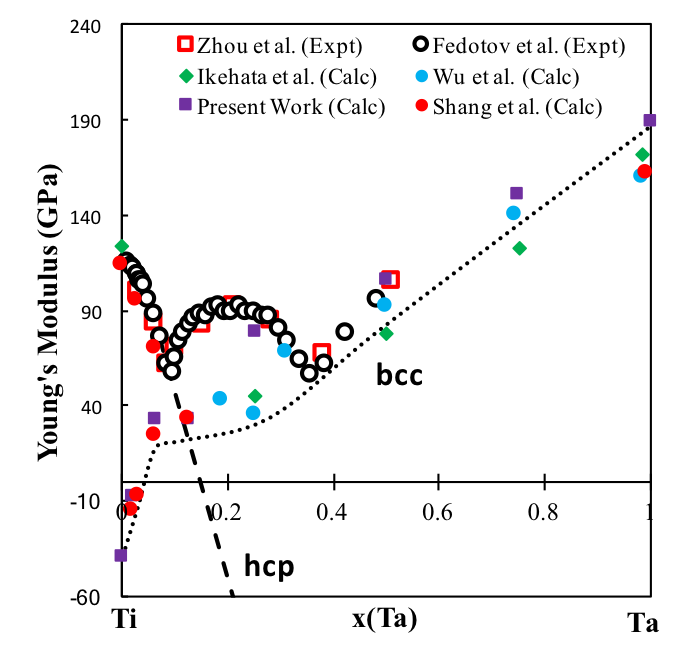
\includegraphics{Chapter-1/Figures/TiTaElastic.png}
	\caption{Comparison of first-principles calculations \cite{Wu2010a,Ikehata2004} and experimental measurements of the Young's moduli of Ti-Ta alloys \cite{Zhou2004a,Zhou2009a,Fedotov1985}. From 0.10 to 0.35 x(Ta) the calculations and experimentally determined $E$ do not match up due to the formation of two metastable phases $\omega$ and $\alpha"$}
	\label{Ch1-figure:titaelastic}
\end{figure}
%%%

\newpage
%%%
\begin{figure}[H]
	\centering
	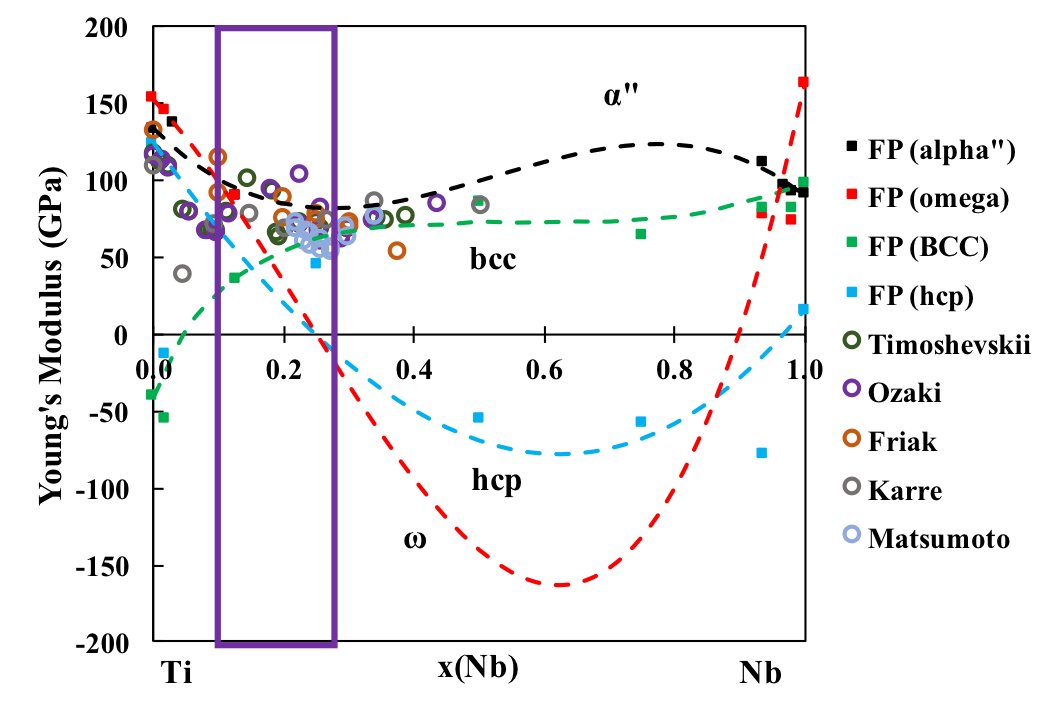
\includegraphics[width=\textwidth]{Chapter-1/Figures/TiNbElastic.png}
	\caption{Comparison of the present first-principles calculations and experimental measurements of the Young's moduli of Ti-Nb alloys \cite{Timoshevskii2011,Ozaki2004,Friak2012,Karre2015,Matsumoto2006}. From 0.10 to 0.30 x(Nb) the calculations and experimentally determined $E$ do not match up due to the formation of two metastable phases $\omega$ and $\alpha"$}
	\label{Ch1-figure:tinbelasitc}
\end{figure}
%%%
